%    Copyright (c) 2008-2010, 2012-2016 Russell V. Lenth

\documentclass[article,nojss]{jss}
\usepackage{amsmath}

%%%% FIX THESE WHEN YOU REVISE! %%%%%%%%%%%%%%%%
\def\VERSION{2.00}
\def\DATE{3 December 2012}
%%%%%%%%%%%%%%%%%%%%%%%%%%%%%%%%%%%%%%%%%%%%%%%%

\def\rsm{\pkg{rsm}}
\def\R{\proglang{R}}
\def\Sect#1{Section~\ref{#1}}
\def\bx{\mathbf{x}}
\def\yhat{\hat{y}}

%% need no \usepackage{Sweave}

\IfFileExists{upquote.sty}{\RequirePackage{upquote}}{}
\DefineShortVerb{\"}

%\VignetteIndexEntry{Surface Plots in the rsm Package}
%\VignetteDepends{rsm}
%\VignetteKeywords{response-surface methods, regression, contour plots, perspective plots}
%\VignettePackage{rsm}

\author{Russell V.~Lenth\\The University of Iowa}
\Plainauthor{Russell V. Lenth}

\title{Surface Plots in the \pkg{rsm} Package\\
\normalsize Updated to version \VERSION, \DATE}
\Plaintitle{Surface Plots in the \pkg{rsm} Package}

\Abstract{
  This is a companion to the main vignette for the \rsm{} package,
  providing more details on how to use the \texttt{contour},
  \texttt{image}, and \texttt{persp} to visualize fitted response surfaces.  While designed with \texttt{rsm} objects in mind, these methods work with any \texttt{lm} object and thus provide a quick way to graph a fitted surface.  Enhancements include coloring, adding contour lines to perspective plots, and hooks that provide additional annotations.
}

\Keywords{response-surface methods, regression, contour plots, perspective plots}

\Address{
  Russell V.~Lenth\\
  Department of Statistics\\
  The University of Iowa\\
  Iowa City, IA 52242, United States of America\\
  E-mail: \email{russell-lenth@uiowa.edu}\\
  URL: \url{http://www.stat.uiowa.edu/~rlenth/}
}


\begin{document}

\section{Introduction}
When a regression model is fitted using two or more continuous predictors, it is useful to present a graphical visualization of the fitted surface.  
To this end, the functions "contour.lm", "persp.lm" and "image.lm" were developed and incorporated in the \rsm{} package, inasmuch as surface visualization is especially important when using response-surface methods.  The three functions are S3 methods for objects of class "lm", or classes (such as "rsm") that inherit from "lm".

This vignette is not meant to document the functions; please refer to the help pages for details.  Our goal here is to illustrate their use.

\section{Models with two predictors}
Consider an example using the ubiquitous "swiss" dataset that is standard in \R{}.  Let us fit a model for "Fertility" as a polynomial function of "Agriculture" and "Education":
\begin{Schunk}
\begin{Sinput}
> swiss2.lm <- lm(Fertility ~ poly(Agriculture, Education, degree=2), data=swiss)
\end{Sinput}
\end{Schunk}
The following basic calls illustrate the default results from the three functions.  The results are shown in Figure~\ref{basics}.
\begin{Schunk}
\begin{Sinput}
> library(rsm)
> par(mfrow=c(1,3))
> image(swiss2.lm, Education ~ Agriculture)
> contour(swiss2.lm, Education ~ Agriculture)
> persp(swiss2.lm, Education ~ Agriculture, zlab = "Fertility")
\end{Sinput}
\end{Schunk}
\begin{figure}
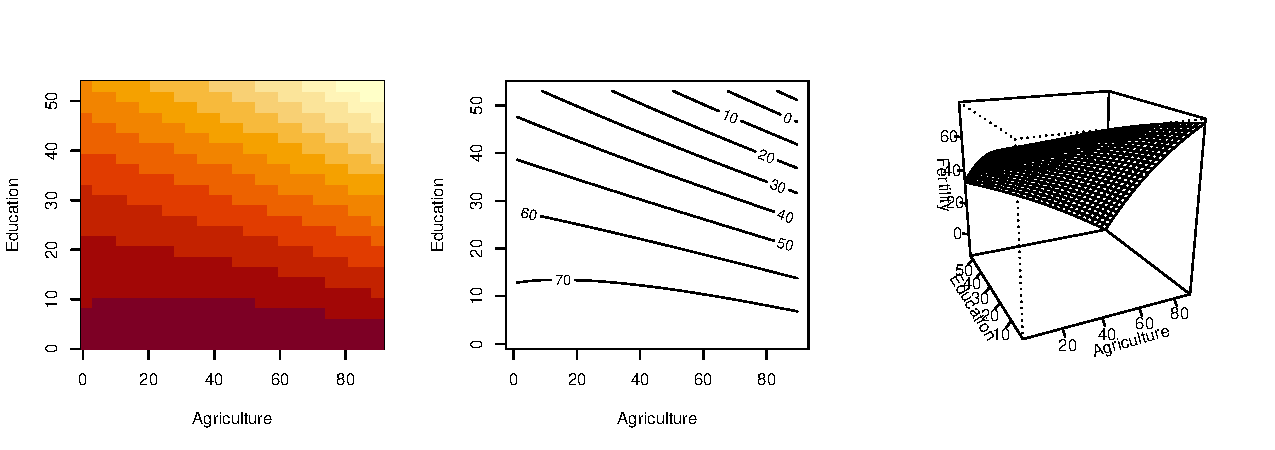
\includegraphics[width=\linewidth, viewport=0 0 583 183, clip]{rsm-plots-basics.pdf}
\caption{Basic image, contour, and perspective plots.}\label{basics}
\end{figure}
Note that we use a formula in the second argument to specify which variable goes on which axis.  The "persp" plot uses a different viewpoint, distance, and tick type than the default; I feel that these new defaults are better for viewing response surfaces.

Generally (as we can see in Figure~\ref{basics}), perspective plots are best not displayed in too small a space.  It also helps to enhance them with shading, colors, or contour lines.  The following call illustrates how to create an enhanced version of the perspective plot with a different point of view, shading, a different surface color, and contour lines added to the top surface of the box.  We also restrict the predictor values to narrower ranges.  The results are shown in Figure~\ref{lessbasic}.
\begin{figure}
\[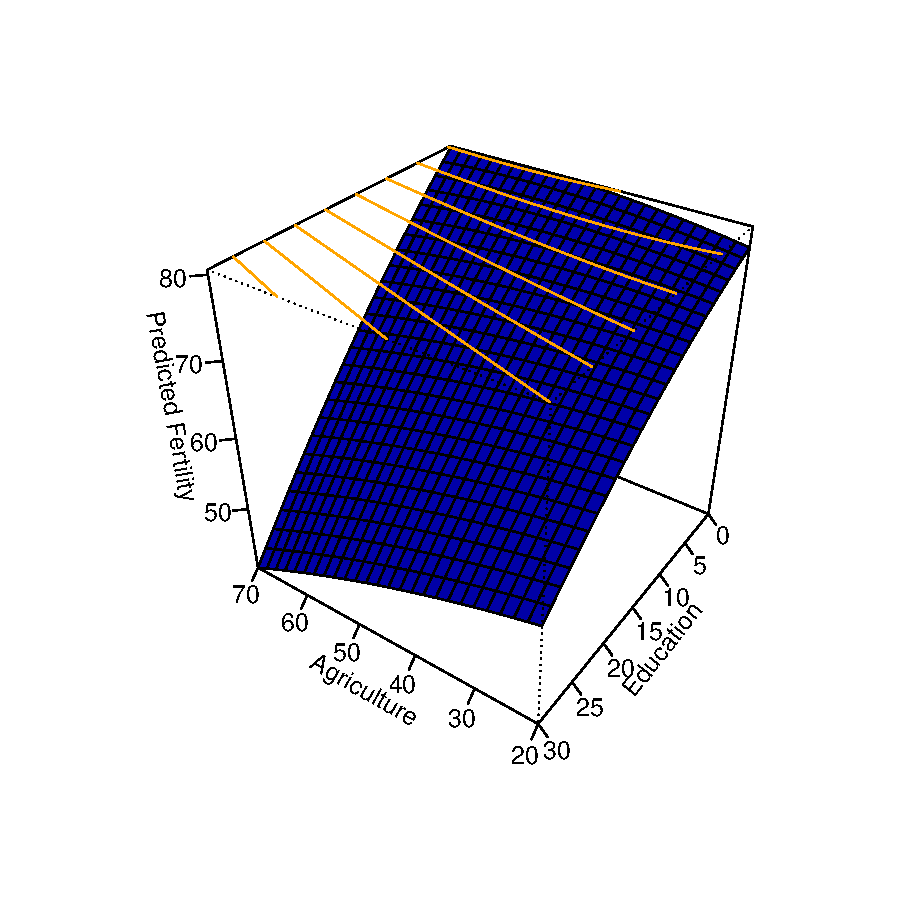
\includegraphics[width=.5\linewidth, viewport=70 60 370 370, clip]{rsm-plots-lessbas.pdf}\]
\caption{Enhanced perspective plot.}\label{lessbasic}
\end{figure}
\begin{Schunk}
\begin{Sinput}
> persp(swiss2.lm, Education ~ Agriculture, col = "blue", 
+   bounds = list(Agriculture=c(20,70), Education=c(0,30)),
+   zlab = "Predicted Fertility", contours = list(z="top", col="orange"), 
+   theta = -145, phi = 35, shade = 1)
\end{Sinput}
\end{Schunk}

\section{Three or more predictors}
When a regression model has more than two continuous predictors, some additional issues arise:
\begin{enumerate}
\item We can use only two predictors at a time in an image, contour, or surface plot.
\item For two given predictors, the surface plot will change depending on the values of the other predictors.  (The defaults for "image", "contour", and "persp" is to use the average, but this can be changed.)
\item There will be more than one surface plot; it is desirable to keep the scaling and coloring consistent among all these plots.  (This happens automatically in all three functions; there is no way to defeat it other than by manually plotting the retrieved surface data.)
\end{enumerate}

For illustration, we will use the data from a paper-helicopter experiment described in \cite{Box05}, page~499, and provided in the \rsm{} package as the dataset "heli".  The variables are coded variables $x_1$--$x_4$, which are, respectively, linear functions of wing area $A$, wing length ratio $R$, body width $W$, and body length $L$.  the experiment was run in two blocks, and the response variable is "ave", the average flight time in seconds.  This dataset is analyzed in more detail in  the \href{rsm.pdf}{main \rsm{} vignette}.  A second-order response-surface model for these data is obtained using
\begin{Schunk}
\begin{Sinput}
> heli.rsm <- rsm(ave ~ block + SO(x1,x2,x3,x4), data = heli)
\end{Sinput}
\end{Schunk}
An "rsm" object is an extension of a "lm" object with extra response-surface-related information included.
To obtain contour plots with each of the 6 possible pairs of the variables $x_1$--$x_4$, simply specify the formula "~ x1 + x2 + x3 + x4" in the call to "contour":
\begin{figure}
\begin{center}
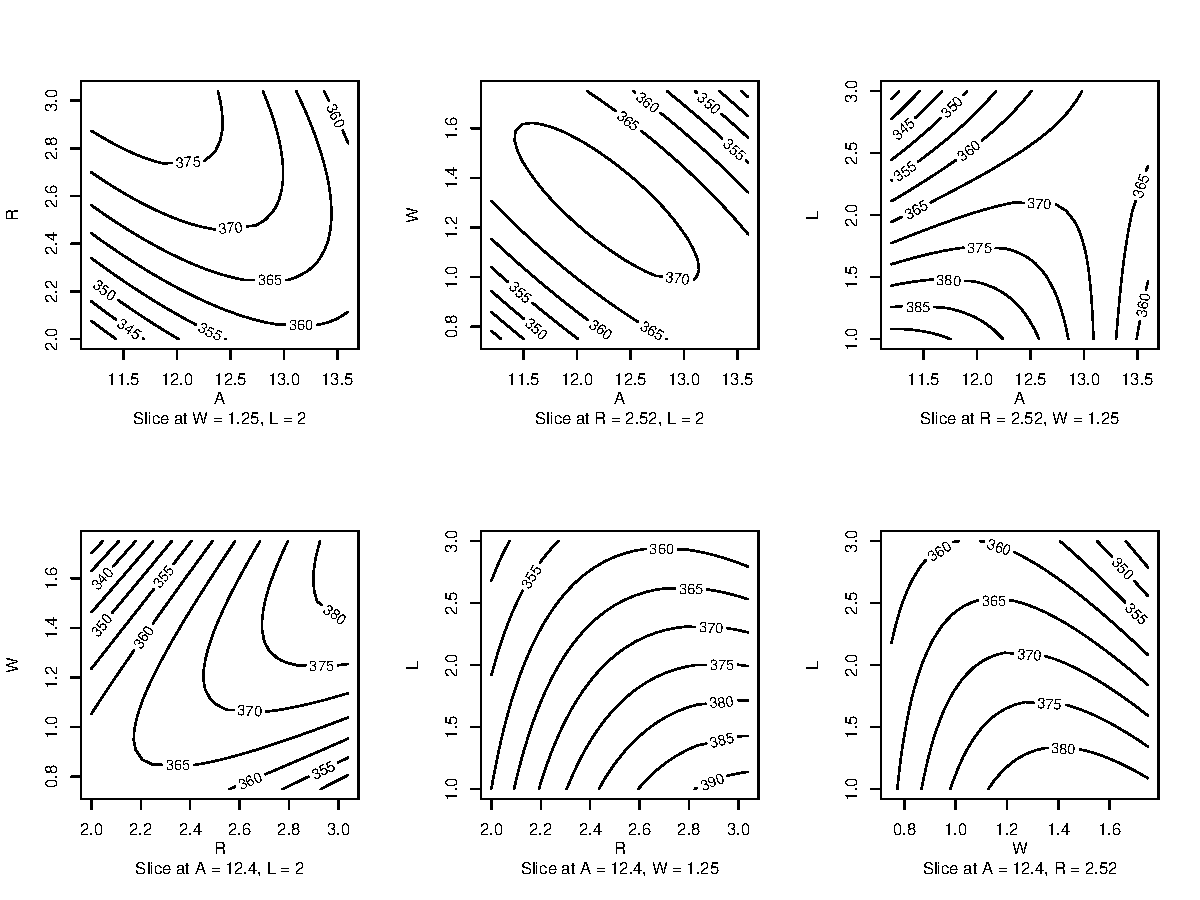
\includegraphics[width=.95\linewidth, viewport=0 10 560 396, clip]{rsm-plots-cont1.pdf}
\end{center}
\vspace{-26pt}
\caption{Default contour plots of \texttt{heli.rsm}.}\label{cont1}
\begin{center}
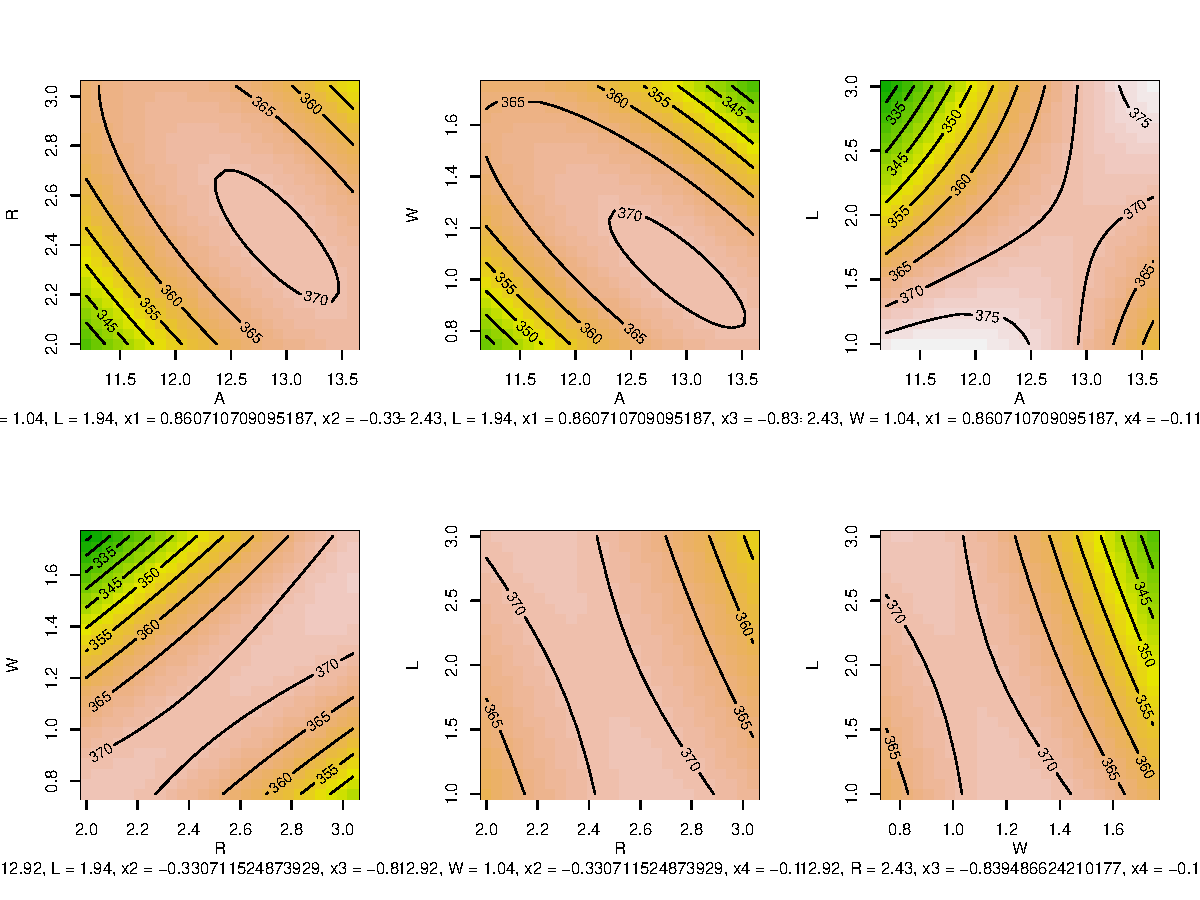
\includegraphics[width=.95\linewidth, viewport=0 10 560 422, clip]{rsm-plots-cont2.pdf}
\end{center}
\vspace{-26pt}
\caption{Enhanced contour plots of \texttt{heli.rsm}.}\label{cont2}
\end{figure}
\begin{Schunk}
\begin{Sinput}
> par(mfrow = c(2,3))
> contour (heli.rsm, ~ x1 + x2 + x3 + x4)
\end{Sinput}
\end{Schunk}
The result is shown in Figure~\ref{cont1}.  This dataset is an extension of "data.frame" that contains the coding information, and this information is retained in "heli.rsm".  When such coding is present, then by default, the coding formulas are used to decode the axis values $x_1,x_2,x_3,x_4$ to their original values $A,R,W,L$.

Also, when variables other than those on the coordinate axes are involved, then what is displayed is a slice of the response surface, holding the other variables fixed at certain values.  By default, we use the averages of numeric predictors, and the first levels of factors.  This information is incorporated as part of the $x$-axis label in each contour plot.
\def\xbar{\bar{x}}
In this example, we are probably more interested in the behavior of the response surface in a neighborhood of the stationary point (where the gradient is zero).  We show how to do this after a little bit more discussion in the next section.

%%%%%If the stationary point is saved as "xs", we simply add the argument "at = xs" in the call to "contour" to center the plots around the stationary point.  This is illustrated in the next section.

\section{Annotations and hooks}
Suppose in the helicopter example, we want to add some annotations to the plots.  Since there are several plots, we don't want to do this manually.  The "contour" method for "lm" objects (as well as "image" and "persp") allow one to specify a "hook" argument to take care of things like that.  The hook should be a "list" containing function definitions for one or both of "pre.plot" and "post.plot".  Obviously, these are functions that are run just before, and just after, each plot is constructed.  Each function is passed one argument, a character vector of length $4$; elements $1$ and~2 are the labels for the horizontal and vertical axes; elements $3$ and~$4$ are the corresponding variable names; and element 5 is a label describing the slice being plotted.

In the following code, we set up a "post.plot" hook to plot the position of the stationary point in each graph.
\begin{Schunk}
\begin{Sinput}
> xs <- canonical(heli.rsm)$xs
> myhook <- list()
> myhook$post.plot <- function(lab) {
+   idx <- sapply(lab[3:4], grep, names(xs))
+   points (xs[idx[1]], xs[idx[2]], pch=2, col="red")
+ }
\end{Sinput}
\end{Schunk}
The coding is a bit tedious due to the need to match elements of "xs" with the variable names.  
To create an enhanced contour plot, use the "at" argument to specify that we want the plots sliced at the stationary point instead of the origin, the "image" argument to enhance the plots with a background color image, and use "hook" to incorporate the above hook function.  
Figure~\ref{cont2} shows the results.
Centering at the stationary point gives an entirely different view of the fitted surface than is seen in Figure~\ref{cont1}.
\begin{Schunk}
\begin{Sinput}
> par(mfrow = c(2,3))
> contour (heli.rsm, ~ x1 + x2 + x3 + x4, image = TRUE,
+   at = xs, hook = myhook)
\end{Sinput}
\end{Schunk}


\section{Saving graphs separately}
An issue comes up when we don't want to squeeze all the plots into one multi-panel frame.  For PostScript and PDF formats, this is easy to handle.  For example:
\begin{Schunk}
\begin{Sinput}
> pdf(file = "heli-cps.pdf")
> contour (heli.rsm, ~ x1 + x2 + x3 + x4, image = TRUE, at = xs, hook = myhook)
> dev.off()
\end{Sinput}
\end{Schunk}
With this example, the resulting file will have six pages, one per graph.  We can then import, say, the fourth graph into a \proglang{pdflatex} source file using a command like
\begin{verbatim}
\includegraphics[width=.75\linewidth, page=4]{heli-cps.pdf}
\end{verbatim}
If you are using \pkg{Sweave}, the device setup is already done in the background, and all you need to do is label the code chunk and import the desired graph(s).


If instead you want to create a separate file for each graph, use hooks to create files based on variable names.  For example,
\begin{Schunk}
\begin{Sinput}
> png.hook <- list()
> png.hook$pre.plot <- function(lab) 
+     png(file = paste(lab[3], lab[4], ".png", sep = ""))
> png.hook$post.plot = function(lab)
+     dev.off()
> contour (heli.rsm, ~ x1 + x2 + x3 + x4, image = TRUE, at = xs, hook = png.hook)
\end{Sinput}
\end{Schunk}
%%%(To also include the titles and annotations, use the "post.plot" function in "myhook", but add the "dev.off()" statement to the end.)

\section{More on perspective plots}
The "lm" method for "persp" handles its "col" argument differently than the default "persp" function.  For other than a single color, it determines surface-facet colors based on the fitted response value (like is done in "image") rather than requiring a matrix of facet colors.

\paragraph{Contours}
To add contour lines to a perspective plot, use the "contours" argument.  It may be a boolean value, character value, or a list.  With "contours=TRUE" or equivalently, \verb|contours="bottom"|, contour lines are drawn on the bottom surface of the box using the default foreground color.  With \verb|contours="top"|, they are drawn at the top.  Bottom contours are drawn before the surface is drawn (so they may become partially obscured), and top contours are drawn afterward.
A value of \verb|contours="colors"| will draw the contours on the bottom, using the same colors as the corresponding contour levels on the surface (as illustrated in Figure~\ref{persp}).  Any other character value of "contours" will be taken as a color name for the contours, e.g., \verb|contours="green"|.  For more control, "contours" can be a list containing any or all of "col" (which may be either \verb|"colors"| or a valid color), "z" (which may be \verb|"top"|, \verb|"bottom"|, or a numeric $z$ value), and "lwd" (to control the width of the lines).

\begin{figure}
\includegraphics[width=.5\linewidth,page=2]{rsm-plots-persp.pdf}%
\includegraphics[width=.5\linewidth,page=3]{rsm-plots-persp.pdf}
\caption{The first and third perspective plots with rainbow colors and contour coloring.}\label{persp}
\end{figure}
\paragraph{Colors}
The plots depicted in Figure~\ref{persp} are two (the first and third of the perspective plots produced by
\begin{Schunk}
\begin{Sinput}
> persp (heli.rsm, ~ x1 + x2 + x3 + x4, at = xs, 
+   col = rainbow(50), contours = "colors")
\end{Sinput}
\end{Schunk}
The plots were saved in a six-page PDF file as described earlier, and pages 1 and~3 were imported to this document.

\section{Doing it your own way}
If these functions do not produce exactly the plot you want, you may still be able to save yourself a lot of work by calling "contour" with the desired object and formula(s), and "plot.it=FALSE".  The returned object is a list of data for each plot---the $x$ and $y$ values, the $z$ matrix, the range of $z$ across all plots, and axis labels.

\bibliography{rsm}

\end{document}
